\documentclass[11pt,a4paper,titlepage]{article}
\usepackage[a4paper]{geometry}
\usepackage[utf8]{inputenc}
\usepackage[english]{babel}
\usepackage{lipsum}

\usepackage{amsmath, amssymb, amsfonts, amsthm, fouriernc, mathtools}
% mathtools for: Aboxed (put box on last equation in align envirenment)
\usepackage{microtype} %improves the spacing between words and letters

\usepackage{graphicx}
\graphicspath{ {./pics/} {./eps/}}
\usepackage{epsfig}
\usepackage{epstopdf}


%%%%%%%%%%%%%%%%%%%%%%%%%%%%%%%%%%%%%%%%%%%%%%%%%%
%% COLOR DEFINITIONS
%%%%%%%%%%%%%%%%%%%%%%%%%%%%%%%%%%%%%%%%%%%%%%%%%%
\usepackage[svgnames]{xcolor} % Enabling mixing colors and color's call by 'svgnames'
%%%%%%%%%%%%%%%%%%%%%%%%%%%%%%%%%%%%%%%%%%%%%%%%%%
\definecolor{MyColor1}{rgb}{0.2,0.4,0.6} %mix personal color
\newcommand{\textb}{\color{Black} \usefont{OT1}{lmss}{m}{n}}
\newcommand{\blue}{\color{MyColor1} \usefont{OT1}{lmss}{m}{n}}
\newcommand{\blueb}{\color{MyColor1} \usefont{OT1}{lmss}{b}{n}}
\newcommand{\red}{\color{LightCoral} \usefont{OT1}{lmss}{m}{n}}
\newcommand{\green}{\color{Turquoise} \usefont{OT1}{lmss}{m}{n}}
%%%%%%%%%%%%%%%%%%%%%%%%%%%%%%%%%%%%%%%%%%%%%%%%%%




%%%%%%%%%%%%%%%%%%%%%%%%%%%%%%%%%%%%%%%%%%%%%%%%%%
%% FONTS AND COLORS
%%%%%%%%%%%%%%%%%%%%%%%%%%%%%%%%%%%%%%%%%%%%%%%%%%
%    SECTIONS
%%%%%%%%%%%%%%%%%%%%%%%%%%%%%%%%%%%%%%%%%%%%%%%%%%
\usepackage{titlesec}
\usepackage{sectsty}
%%%%%%%%%%%%%%%%%%%%%%%%
%set section/subsections HEADINGS font and color
\sectionfont{\color{MyColor1}}  % sets colour of sections
\subsectionfont{\color{MyColor1}}  % sets colour of sections

%set section enumerator to arabic number (see footnotes markings alternatives)
\renewcommand\thesection{\arabic{section}.} %define sections numbering
\renewcommand\thesubsection{\thesection\arabic{subsection}} %subsec.num.

%define new section style
\newcommand{\mysection}{
\titleformat{\section} [runin] {\usefont{OT1}{lmss}{b}{n}\color{MyColor1}} 
{\thesection} {3pt} {} } 

%%%%%%%%%%%%%%%%%%%%%%%%%%%%%%%%%%%%%%%%%%%%%%%%%%
%       CAPTIONS
%%%%%%%%%%%%%%%%%%%%%%%%%%%%%%%%%%%%%%%%%%%%%%%%%%
\usepackage{caption}
\usepackage{subcaption}
%%%%%%%%%%%%%%%%%%%%%%%%
\captionsetup[figure]{labelfont={color=Turquoise}}

%%%%%%%%%%%%%%%%%%%%%%%%%%%%%%%%%%%%%%%%%%%%%%%%%%
%       !!!EQUATION (ARRAY) --> USING ALIGN INSTEAD
%%%%%%%%%%%%%%%%%%%%%%%%%%%%%%%%%%%%%%%%%%%%%%%%%%
%using amsmath package to redefine eq. numeration (1.1, 1.2, ...) 
%%%%%%%%%%%%%%%%%%%%%%%%
\renewcommand{\theequation}{\thesection\arabic{equation}}

%set box background to grey in align environment 
\usepackage{etoolbox}% http://ctan.org/pkg/etoolbox
\makeatletter
\patchcmd{\@Aboxed}{\boxed{#1#2}}{\colorbox{black!15}{$#1#2$}}{}{}%
\patchcmd{\@boxed}{\boxed{#1#2}}{\colorbox{black!15}{$#1#2$}}{}{}%
\makeatother
%%%%%%%%%%%%%%%%%%%%%%%%%%%%%%%%%%%%%%%%%%%%%%%%%%

\definecolor{QuestionColour}{RGB}{45, 135, 51}

\newcommand{\blankline}{\quad\pagebreak[2]}
\setlength{\parskip}{0.3em}

%%%%%%%%%%%%%%%%%%%%%%%%%%%%%%%%%%%%%%%%%%%%%%%%%%
%% DESIGN CIRCUITS
%%%%%%%%%%%%%%%%%%%%%%%%%%%%%%%%%%%%%%%%%%%%%%%%%%
\usepackage[siunitx, american, smartlabels, cute inductors, europeanvoltages]{circuitikz}
%%%%%%%%%%%%%%%%%%%%%%%%%%%%%%%%%%%%%%%%%%%%%%%%%%



\makeatletter
\let\reftagform@=\tagform@
\def\tagform@#1{\maketag@@@{(\ignorespaces\textcolor{red}{#1}\unskip\@@italiccorr)}}
\renewcommand{\eqref}[1]{\textup{\reftagform@{\ref{#1}}}}
\makeatother
\usepackage{hyperref}
\hypersetup{colorlinks=true}

%%%%%%%%%%%%%%%%%%%%%%%%%%%%%%%%%%%%%%%%%%%%%%%%%%
%% PREPARE TITLE
%%%%%%%%%%%%%%%%%%%%%%%%%%%%%%%%%%%%%%%%%%%%%%%%%%
\title{\blue INFOSYS 722 \\
Data Mining and Big Data \\
\blueb Iteration $IV$}
\author{Jason Tam}
\date{\today}
%%%%%%%%%%%%%%%%%%%%%%%%%%%%%%%%%%%%%%%%%%%%%%%%%%



\begin{document}
\maketitle

\section{Business and/or Situation understanding}

The United Nations General Assembly has adopted the 2030 Agenda for Sustainable Development with 17 \href{https://www.un.org/development/desa/disabilities/envision2030.html}{\textbf{Sustainable Development Goals}} in September 2015, as shown in Figure \ref{fig:UNGoals}. These goals are established based on the principle of "leaving no one behind", which aims to include persons with disabilities in the development process, creating a sustainable world that is truly better for everyone.

\blankline

\begin{figure}[!htbp]
    \begin{center}
        
\includegraphics[width=0.8\textwidth]{UNGoals.png}
        \caption{Sustainable Development Goals from the 2030 Agenda for Sustainable Development that was adopted by the United Nations General Assembly in September 2015.}
        \label{fig:UNGoals}
    \end{center}
\end{figure}
 
While the actions to counter the effects of climate change may be categorized under the ‘Climate Action’ goal, its influence does spread to many other goals such as “Clean Water and Sanitation” and “Affordable and Clean Energy”. This makes it one of the most important issues that needs to be studied in depth to determine effective and efficient measures to counter the effects. 

\blankline

Emissions of carbon dioxide (CO2) has been identified as one of the main drivers of climate change. Modernization via industrialization has dramatically improved the quality of life in many countries in the last century, with CO2 being linked closely as a bi-product. Identifying countries with relatively low emissions while maintaining decent economy would act as a good starting point for this study, which would assist in identifying effective approaches in various aspects such as recycling and the use of environmentally sustainable energy sources that can be used as examples for other counties. This studies aims to determine if there is a general relationship between the CO$_{2}$ emissions and the other relevant quantities including forest area percentage, total and urban population, as well as Gross Domestic Product (GDP) data of the countries listed. The obtained results may help to indicate if on optimal balance of these quantities exist to produce a thriving economy while maintaining low CO$_{2}$ emissions.

\blankline

The analysis described in this report was performed following the schedule presented in Table \ref{ProjectPlan}, where week number refers to the week numbers of Semester 2 of University of Auckland's 2018 academic calendar.

\begin{table}[htbp!]
    \begin{center}
        \begin{tabular}{ |c|c| } 
        \hline
        Time (Week No.) & Task \\ 
        \hline
        1 & Business Understanding \\
        2 & Data Searching \\
        3 & Data Exploration \\
        4 & Data Preparation \\
        5 & Data Mining \\
        6 & Model Tuning \\
        7 & Results Visualization \\
        8 & Report Writing \\
        \hline
        \end{tabular}
        \caption{Time plan for analysis}
        \label{ProjectPlan}
    \end{center}
\end{table}

% \pagebreak
\section{Data understanding}

\blankline

The \href{https://www.worldbank.org/}{World Bank} contains comprehensive data sets on various macro-economic variables for a list of countries that are available for download. Historical data for some more developed countries is available further back in time compared to the others, while otherwise being reasonably comprehensive and complete. Global data of relevant variables such as population, urban population, CO2 emission, Gross Domestic Product (GDP) and forest area were obtained from the website, and each of them were available in independent comma separated (CSV) files with a common structure. Five CSV files where downloaded under the 'Climate Change' category under the \href{https://data.worldbank.org/indicator}{World Development Indicators} section of the World Bank website, which contains time series data for each of the following variables:

\begin{itemize}
    \item{Gross Domestic Product (GDP)}
    \item{Total population}
    \item{Urban population as a percentage of total}
    \item{Forest area as a percentage of total land area}
    \item{CO$_2$ emissions (tonnes)}
\end{itemize}

The available data for each of the variables are presented as annual figures from 1960 to 2017, for a list of "countries" that are listed in \texttt{countryTypeDict.txt} in the \textit{Code} directory. The data for each year is presented in columns, while each of the "countries" in the list occupies a row. This list of "countries" contain all countries that are recognized by the United Nations, as well as entries that represent a group of countries that share some common attributes, such as \texttt{Central Europe and the Baltic's} and \texttt{Caribbean small states}. These group entries are excluded from this analysis to avoid the overlap of statistics.

\blankline

\href{https://www.python.org/}{Python} and associated open source libraries such as \href{https://pandas.pydata.org/}{Pandas} are used in this instance for the analysis. The python codes that have been written for this analysis are stored in the \textit{Code} directory. Written functions are split accordingly into four different files:

\begin{itemize}
    \item \texttt{DataAnalysis.py} - Main executing code.
    \item \texttt{FitFunctions.py} - Contains functions for statistical fitting
    \item \texttt{DFFunctions.py} - Contains functions for dataframe operations
    \item \texttt{plotAnalysis.py} - Contains functions for creating plots
\end{itemize}

These CSV files are loaded into dataframe objects with the \texttt{getCSVDF} function in \texttt{FitFunctions.py}. Dataframe objects are common in analysis work with programming languages such as \href{https://www.r-project.org/}{\texttt{R}} and Python, as they are much like ordinary tables that stores structured data in the rows and columns format, with capabilities of joining to other dataframes in multiple ways that are analogous to tables in relational databases. In Python they are loaded from the Pandas library, which also contains many associated functions that are useful in manipulating the dataframes during the analysis process. 

\blankline

While some of the datasets are complete up to the year 2017, others such as forest land percentage and CO$_{2}$ emissions only have complete data up to 2014. Data in the years beyond 2014 are missing for some countries, particularly the smaller states. As the scope of this analysis does not require a time-dependent element, the data from the year 2013 will be used to train the models, while the 2014 set will be used to evaluate the model.

\section{Data Preparation}

The listed countries are arranged in rows of the dataframe. Names and codes for each of them are provided as columns, as well as the name and code for the data variable. Yearly value of the variable for each year is arranged in a separate column, with the value associated to the respective country at each row. The full list of 'countries' provided in all of the CSV files are identical, which some entries are group entities with definitions that includes multiple nations. A Python dictionary was created to differentiate the standalone nations from the group entities, which is stored in the \texttt{countryTypeDict.txt} file in the same directory. It is loaded into the code through the \texttt{DFFunctions.py} class. After filtering out the group entities, there are 216 entries remaining as standalone 'countries'. Closer inspections has revealed some of the entries are independent territories of a bigger nation such as \textit{Hong Kong SAR}, which explains the 216 entries of 'countries' while there are only 195 officially recognized by the \href{http://www.un.org/en/index.html}{United Nations}.

\blankline

The 216 independent entries for this category makes it difficult to visualize data of any of the quantities for all of them simultaneously. Displaying the top 20 entries for each of the quantity has chosen to be an initial approach.

\blankline

Figure \ref{fig:LandForest2013} shows the top 20 entries for percentage of forest area. It can be observed that with the exception of Finland, Malaysia, Japan and Sweden, the rest of the entries are all small nations that commonly would not be categorized in the group of most developed nations.

\begin{figure}[!htbp]
    \begin{center}
        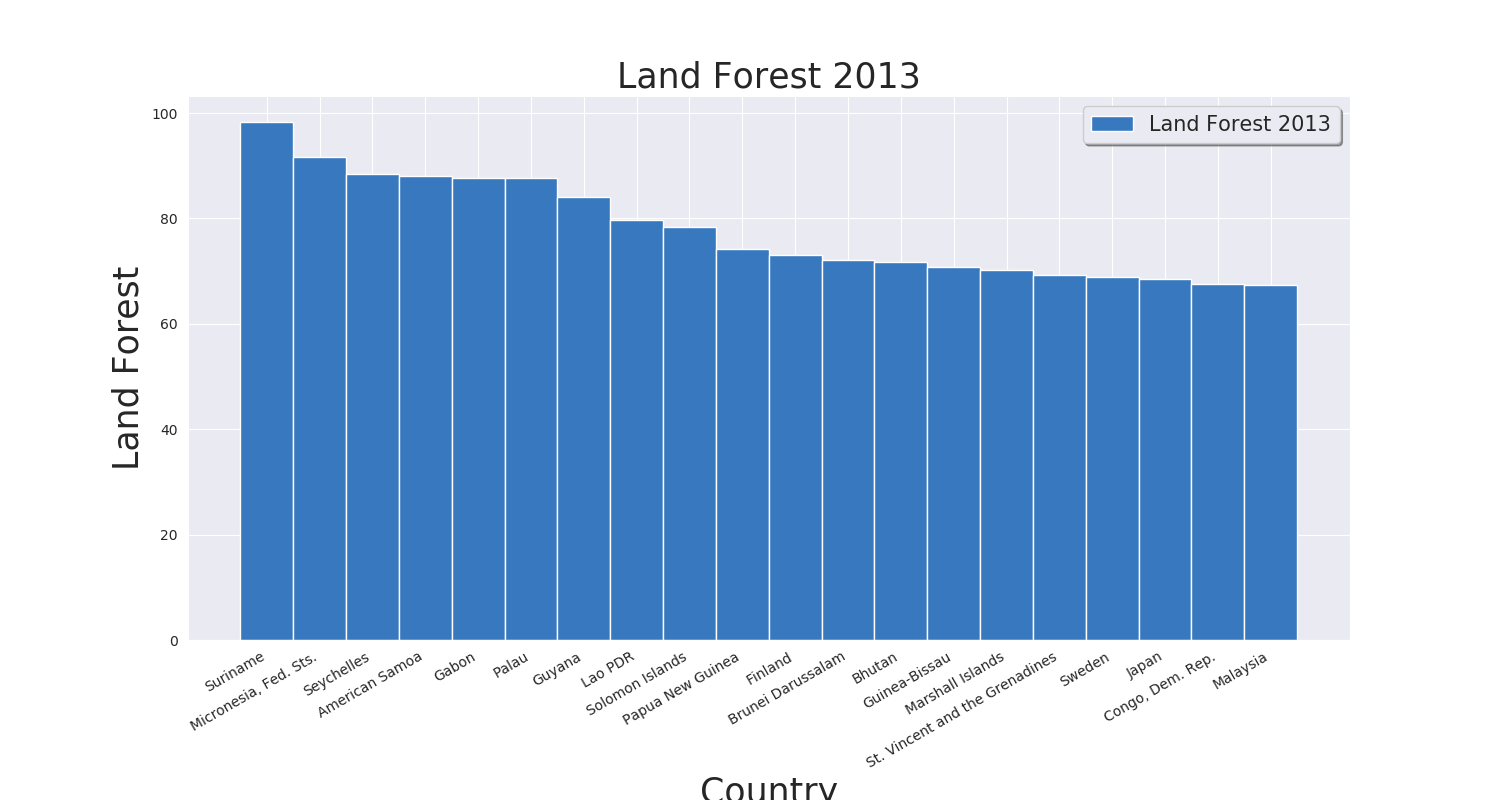
\includegraphics[width=\textwidth]{../Plots/LandForest_2013.png}
        \caption{Land Forest data of top 20 standalone nations for the year of 2013 from the \href{https://www.worldbank.org/}{World Bank}.}
        \label{fig:LandForest2013}
    \end{center}
\end{figure}

\blankline

Figures \ref{fig:CO22013} and \ref{fig:GDP2013} respectively shows the top 20 entries for CO$_{2}$ emissions and GDP data. It can be observed that there are some common entries in both lists, such as the United States, China, Germany, Russia, Brazil and South Korea. In fact with the exception of Spain and Switzerland, the rest of the top 20 nations in GDP are also in the top 20 list for CO2. With both graphs being in similar shape, it can be assumed that there is high potential that there exist a correlation between these two quantities.

\begin{figure}[!htbp]
    \begin{center}
        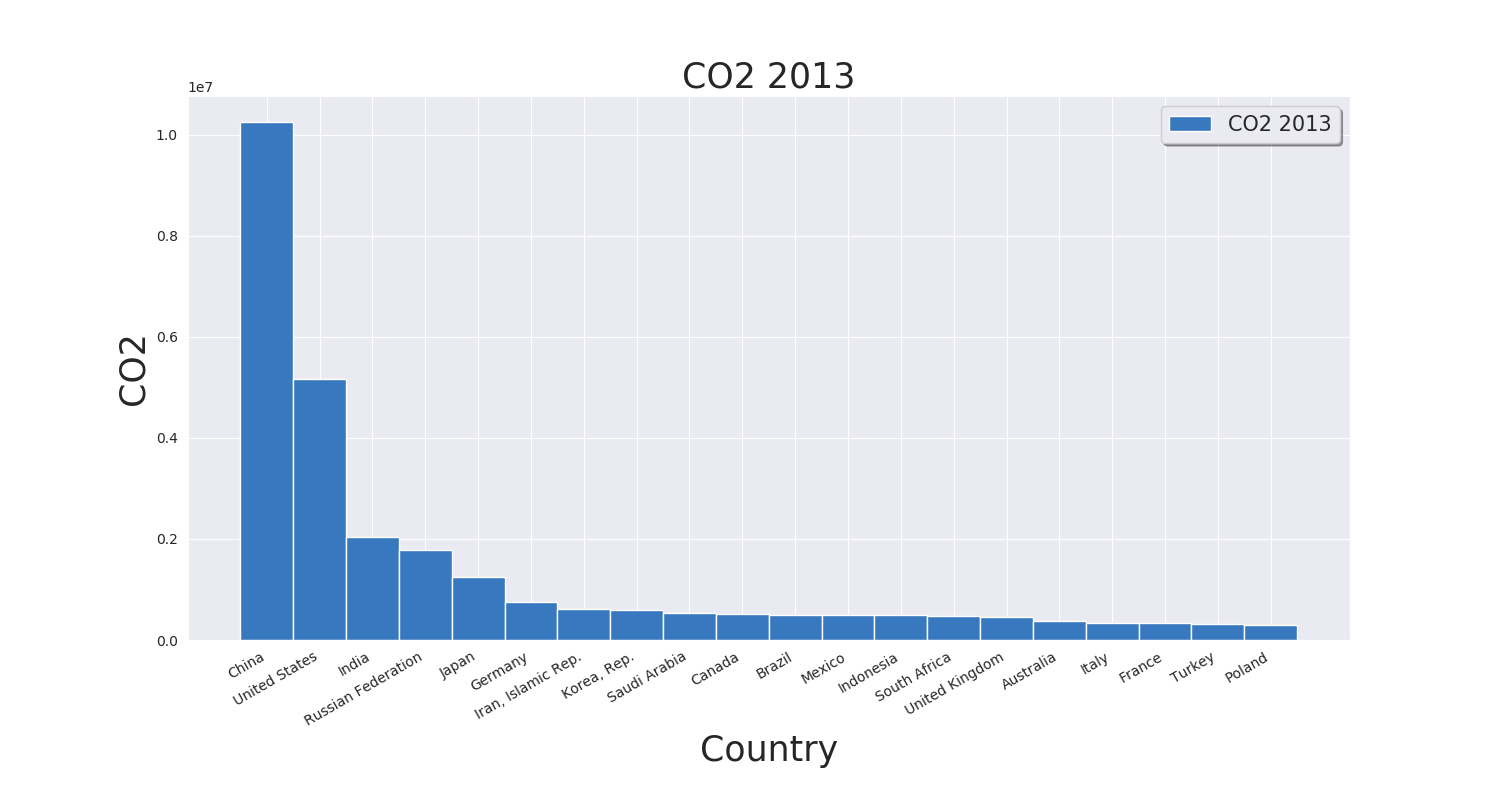
\includegraphics[width=\textwidth]{../Plots/CO2_2013.png}
        \caption{Atmospheric CO$_{2}$ data of top 20 standalone nations for the year of 2013 from the \href{https://www.worldbank.org/}{World Bank}.}
        \label{fig:CO22013}
    \end{center}
\end{figure}

\begin{figure}[!htbp]
    \begin{center}
        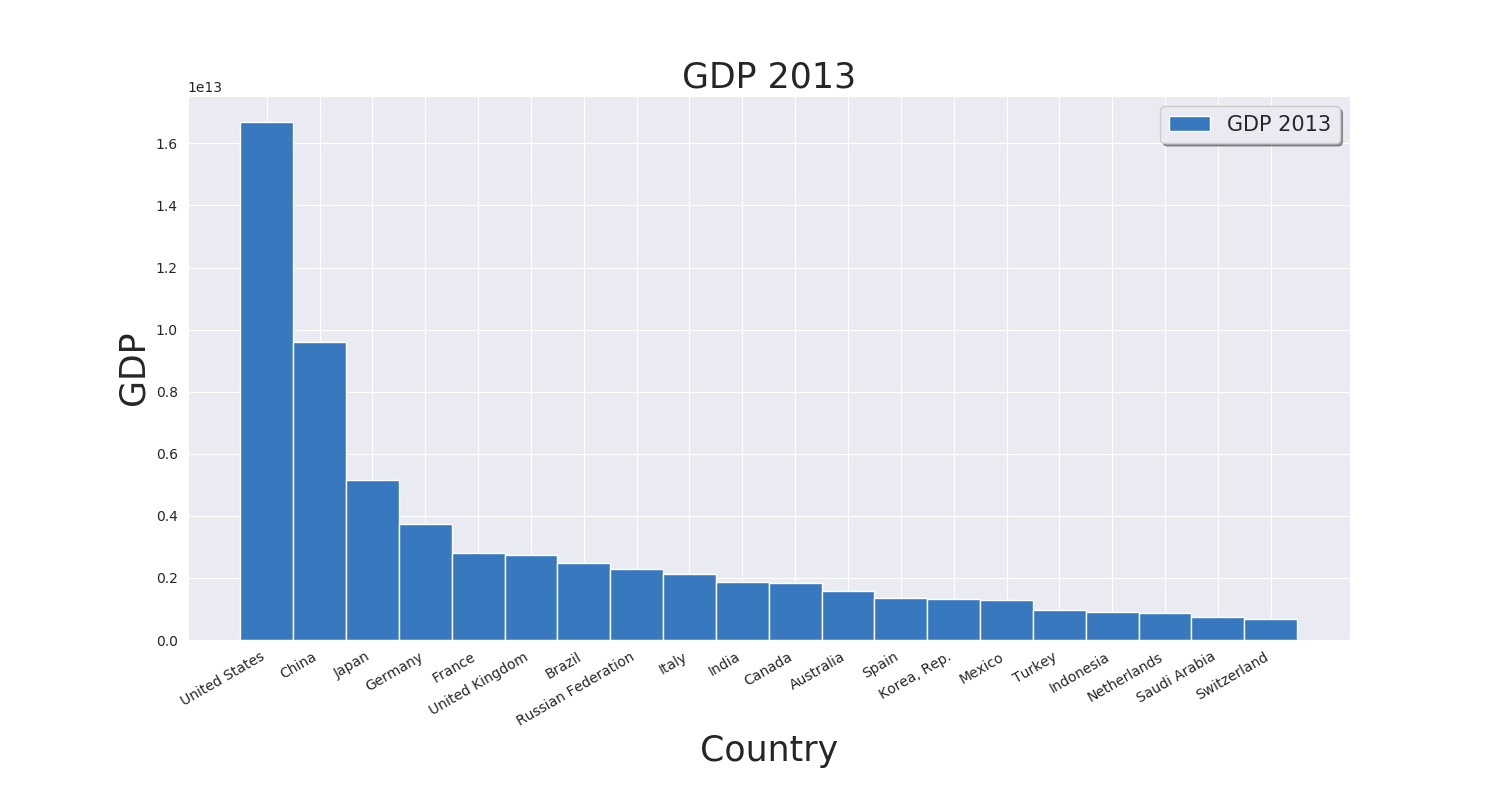
\includegraphics[width=\textwidth]{../Plots/GDP_2013.png}
        \caption{Gross Domestic Product (GDP) data of top 20 standalone nations for the year of 2013 from the \href{https://www.worldbank.org/}{World Bank}.}
        \label{fig:GDP2013}
    \end{center}
\end{figure}

The distribution of the top 20 nations with the most population shares similar shape to the previous two graphs, as shown in Figure \ref{fig:populationTotal2013}. While it can be observed the both Chain and the United States hold the top two spots in all three distributions, the other countries in this list is not as similar to the other two.

\begin{figure}[!htbp]
    \begin{center}
        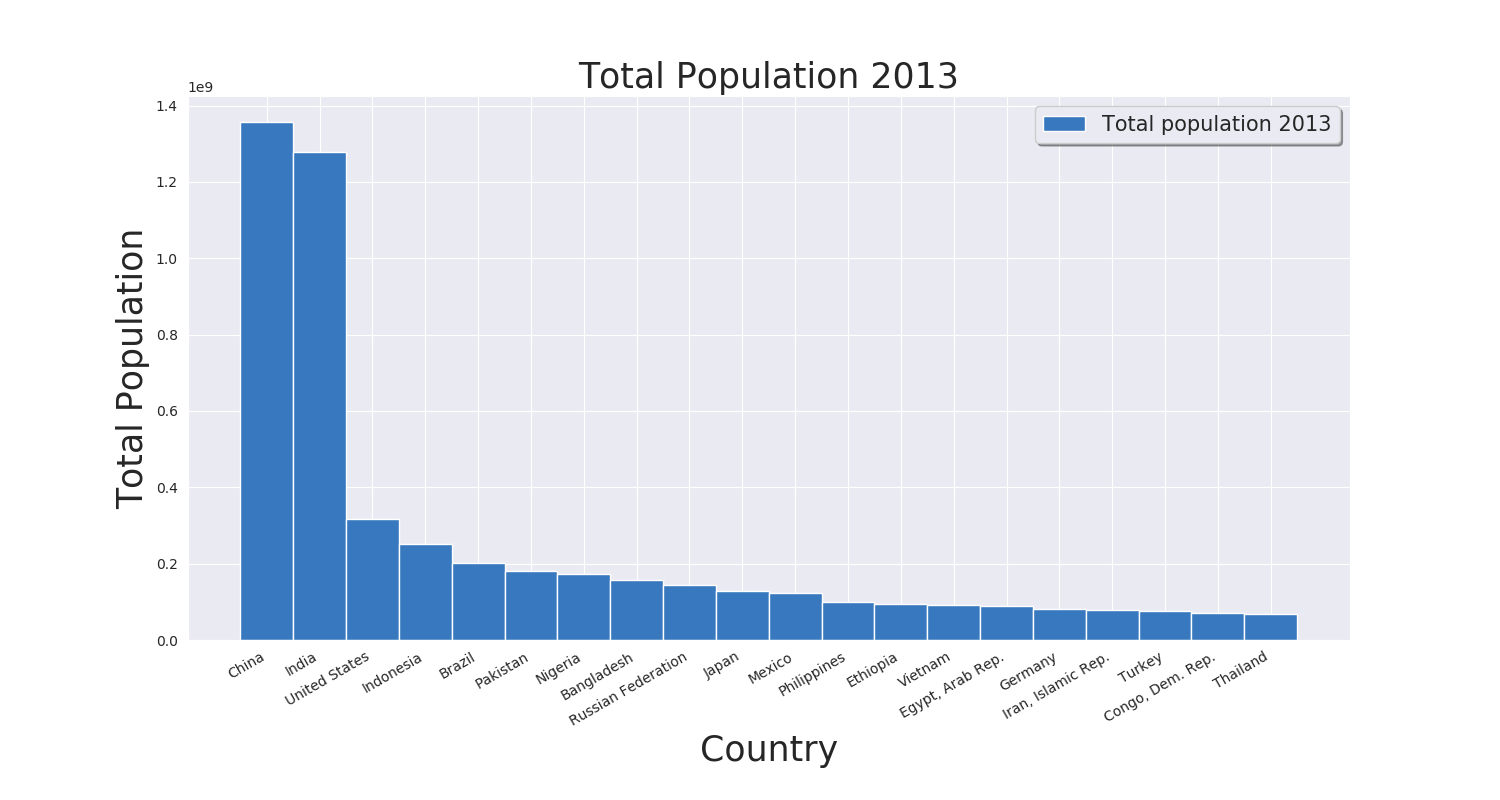
\includegraphics[width=\textwidth]{../Plots/populationTotal_2013.png}
        \caption{Total population data of top 20 standalone nations for the year of 2013 from the \href{https://www.worldbank.org/}{World Bank}.}
        \label{fig:populationTotal2013}
    \end{center}
\end{figure}

Figure \ref{fig:populationUrban2013} shows the distribution of 20 countries with the highest urban population percentage, while Figure \ref{fig:populationUrbanBottom2013} show the bottom 20. It can be observed that most of the countries that make either of these two lists are small nations, which may have little influence on the model.

\begin{figure}[!htbp]
    \begin{center}
        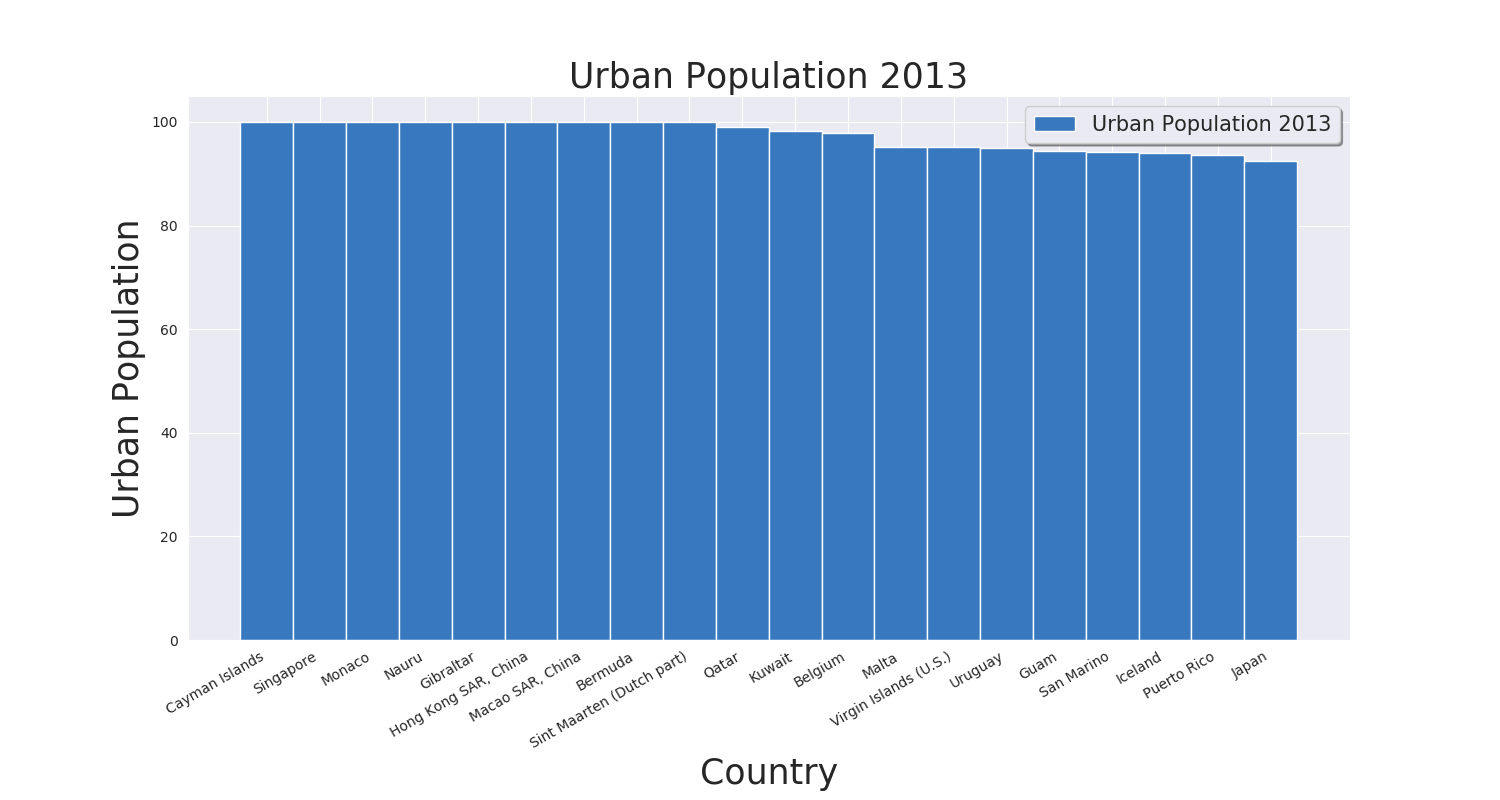
\includegraphics[width=\textwidth]{../Plots/populationUrban_2013.png}
        \caption{Urban population data of top 20 standalone nations for the year of 2013 from the \href{https://www.worldbank.org/}{World Bank}.}
        \label{fig:populationUrban2013}
    \end{center}
\end{figure}

\begin{figure}[!htbp]
    \begin{center}
        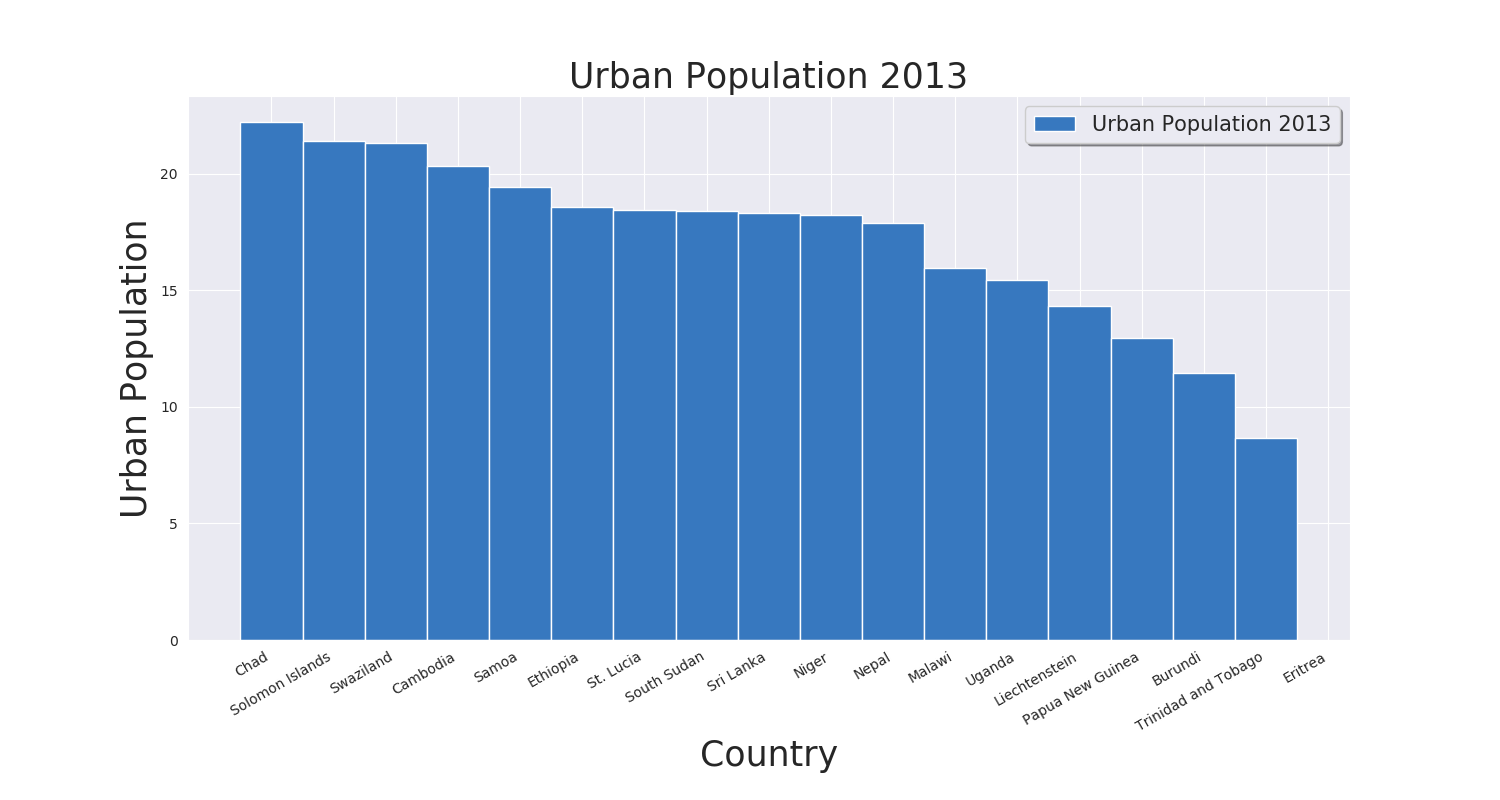
\includegraphics[width=\textwidth]{../Plots/populationUrban_2013_bottom.png}
        \caption{Urban population data of top 20 standalone nations for the year of 2013 from the \href{https://www.worldbank.org/}{World Bank}.}
        \label{fig:populationUrbanBottom2013}
    \end{center}
\end{figure}

\section{Data Transformation}

The columns with 2013 data from each of the dataframes are merged into a single one for analysis. This is performed in the main part of the analysis code (\texttt{DataAnalysis.py}):

\begin{verbatim}
dfList = [self.landForest_DF,
     self.atmosphereCO2_DF,
     self.GDP_DF,
     self.populationTotal_DF,
     self.populationUrban_DF]

trainSetupDF = pd.DataFrame({
    'Country':self.landForest_DF['Country Name'],
    'CountryType':self.landForest_DF['CountryType']
    })
testSetupDF = pd.DataFrame({
    'Country':self.landForest_DF['Country Name'],
    'CountryType':self.landForest_DF['CountryType']
    })

for i in range(0,len(dfList)):
    tempDF = dfList[i]
    # Pick year with data in every variable, particularly atmosphereCO2
    trainSetupDF[dfColumnHeaders[i]] = tempDF['2013']
    testSetupDF[dfColumnHeaders[i]] = tempDF['2014']
\end{verbatim}

\blankline

The group entities are then filtered out using the \texttt{setupAnalysisDF} function in \texttt{DFFunctions.py}. 

\begin{verbatim}
    def setupAnalysisDF(self, inDF, filter=True, countryType='Country'):

        outDF = inDF.copy()

        if (filter==True):
            outDF = outDF[outDF['CountryType']==countryType]

        outDF = outDF.dropna()
        outDF = outDF.reset_index()
        outDF = outDF.drop('index', axis=1)
        # outDF = outDF.set_index('Country')

        return outDF
\end{verbatim}

\blankline

The predictors and targets for both the training data set and the testing data set are defined using the following lines in \texttt{DataAnalysis.py}:

\begin{verbatim}
train_predictors = trainDF.drop([
    'atmosphereCO2',
    'CountryType',
    'Country'], axis=1).copy()
train_target = pd.DataFrame({'atmosphereCO2':trainDF['atmosphereCO2']})

test_predictors = testDF.drop([
    'atmosphereCO2',
    'CountryType',
    'Country'], axis=1).copy()
test_target = pd.DataFrame({'atmosphereCO2':testDF['atmosphereCO2']})
\end{verbatim}

\blankline

Tools from PySpark were used to transform dataframes further for compatibility with modelling functions from PySpark's machine learning library \texttt{MLlib}. \texttt{VectorAssembler} was used to convert the values from each of the predictors from each row into a single vector, which is stored as the value of each cell in a standalone dataframe column, \texttt{"features"} in this case. The resulting dataframe for input contains only this \texttt{features} column and the target column of \texttt{atmosphereCO2}. 

\begin{verbatim}
# Use Vector Assembler to prepare a DF for ML functions

train_DF = self.sql.createDataFrame(trainDF)
test_DF = self.sql.createDataFrame(testDF)

vectorAssembler = VectorAssembler(inputCols = ['landForest', 'populationTotal', \
    'GDP', 'populationUrban'], outputCol = 'features')
trainMLDF = vectorAssembler.transform(train_DF)
trainMLDF = trainMLDF.select(['features', 'atmosphereCO2'])

testMLDF = vectorAssembler.transform(test_DF)
testMLDF = testMLDF.select(['features', 'atmosphereCO2'])
\end{verbatim}

These basic transformations of the data set can be served as input to multiple algorithms of choice for the analysis.

\section{Data-mining Algorithms and Methods Selection}

This analysis with a target prediction quantity of CO$_{2}$ emissions and several predictors such as GDP and population data falls under the \textbf{Supervised Learning} category of the machine learning domain. \textbf{Linear Regression} is a traditional statistical approach under this domain, which attempts to establish a linear relationship between the predictors and the target variable. \textbf{Decision Tree} and \textbf{Gradient Boosted Tree} are machine learning methods that are well known for their abilities in prediction models, which the model is built in general by recursively partitioning the data in a branching out tree manner using different attributes of the data, and the tree structure obtained in the end is used as a prediction model for new data input. These three approaches were performed and their results are used to determine which of them provides the highest level of accuracy for this data set.

\section{Data Mining}

\subsection{Linear Regression}

Linear regression is performed with the training data, using tools from the \texttt{PySpark} package, in the function \texttt{FitLinearRegression} in \texttt{DataAnalysis.py}:

\begin{verbatim}
def FitLinearRegression(self, trainMLDF, testMLDF):

    print("Running Linear Regression.....")

    lr = LinearRegression(featuresCol = 'features', labelCol='atmosphereCO2', \
        maxIter=100, regParam=0.3, elasticNetParam=0.8)
    lr_model = lr.fit(trainMLDF)
    print("Coefficients: " + str(lr_model.coefficients))
    print("Intercept: " + str(lr_model.intercept))

    trainingSummary = lr_model.summary
    print("RMSE: %f" % trainingSummary.rootMeanSquaredError)
    print("r2: %f" % trainingSummary.r2)

    trainMLDF.describe().show()

    lr_predictions = lr_model.transform(testMLDF)
    lr_evaluator = RegressionEvaluator(predictionCol="prediction", \
        labelCol="atmosphereCO2",metricName="r2")
    print("R Squared (R2) on test data = %g" % lr_evaluator.evaluate(lr_predictions))

    test_result = lr_model.evaluate(testMLDF)
    print("Linear Regression Root Mean Squared Error (RMSE) on test data = %g" \
        % test_result.rootMeanSquaredError)

    print("numIterations: %d" % trainingSummary.totalIterations)
    print("objectiveHistory: %s" % str(trainingSummary.objectiveHistory))

    return
\end{verbatim}

The following results were obtained for the training data set:

\begin{verbatim}
Coefficients: [-248.34916025386633,0.0031732740535042685,\
    3.0164649560364597e-07,-1.7513975685464267]
Intercept: -54489.9922589
RMSE: 335665.319288
r2: 0.845423
\end{verbatim}

The coefficients for each of the predictors are presented in the following table:

\begin{table}[htbp!]
    \begin{center}
        \begin{tabular}{ |c|c| } 
        \hline
        Predictor & Coefficient (3d.p.) \\ 
        \hline
        \texttt{landForest} & -248.349\\
        \texttt{populationTotal} & 0.003 \\
        \texttt{GDP} & 3.016$\times$10$^{-7}$ \\
        \texttt{populationUrban} & -1.751 \\
        \hline
        \end{tabular}
        \caption{Coefficients obtained from Linear Regression analysis.}
        \label{LinearRegressionCoeffs}
    \end{center}
\end{table}

With an $R^{2}$ values of 0.845, the results suggests reasonable validity of the coefficients obtained. It is not surprising to find such a big negative correlation (-248.349) for forest percentage of the total land area, and and a reasonable relationship with the urban percentage of the total population. It is however a little interesting to find almost no correlation between the amount of CO2 emissions and total population as well as GDP.

The performance of the obtained linear regression model on the test data set is as follows:

\begin{verbatim}
R Squared (R2) on test data = 0.857565
Linear Regression Root Mean Squared Error (RMSE) on test data = 326331
\end{verbatim}

The Root Mean Squared Error (RMSE) value is smaller than the equivalent obtained for the training data set, while the $R^{2}$ value is also higher. This result of the obtain model on the test data indicates that its predictions are even closer to the actual values in the test data set compared to the training data set, which provide confidence on the potential of overfitting issues on the obtained model.

\subsection{Decision Tree}

One of the main differences between traditional statistical approaches and machine learning methods is the concept of training. Machine learning models such as \textbf{Decision Trees} require preset hyper-parameters as boundary conditions, and training of the model essentially means fine tuning of these hyper-parameters to match the predictors optimally with the target response. As an example, the parameter \texttt{minInstancesPerNode} that can be set for the \texttt{DecisionTreeRegressor} function determines the minimum number of data points in a partition. This prevents the algorithm to further divide the partition if the size is below this threshold. The \texttt{DecisionTreeRegressor} tool provided by the PySpark package for regression analysis using decision trees contains a set of default parameters is none is provided when it is executed.

\begin{verbatim}
('maxBins', 32)
Max number of bins for discretizing continuous features.\
Must be >=2 and >= number of categories for any categorical feature.

('minInstancesPerNode', 1)
Minimum number of instances each child must have after split.\
If a split causes the left or right child to have fewer than minInstancesPerNode,\
the split will be discarded as invalid. Should be >= 1.

('maxDepth', 5)
Maximum depth of the tree. (>= 0) E.g., depth 0 means 1 leaf node;\
depth 1 means 1 internal node + 2 leaf nodes.
\end{verbatim}

An iteration with this default setting is performed, while a set of hyper-parameters are also used for further iterations in search of the optimal model:

\begin{verbatim}
dt_maxDepth_array = [10,20,30]
dt_maxBins_array = [32,34,36]
dt_minInstancesPerNode_array = [1,2,3]
\end{verbatim}

These selections of parameters are estimated using the default values, and are iterated through as inputs to the decision tree algorithm to determine the combination for the optimal model:

\begin{verbatim}
dt_results_array = [] # minInstancesPerNode, maxDepth, maxBins, rmse

for i in range(0, len(dt_maxDepth_array)):
    for j in range(0, len(dt_maxBins_array)):
        for k in range(0, len(dt_minInstancesPerNode_array)):
            dt_maxDepth = dt_maxDepth_array[i]
            dt_maxBins = dt_maxBins_array[j]
            dt_minInstancesPerNode = dt_minInstancesPerNode_array[k]

            dt_params = {
                "maxDepth":dt_maxDepth,
                "maxBins":dt_maxBins,
                "minInstancesPerNode":dt_minInstancesPerNode
            }

            dt_results_array.append(self.FitDecisionTree(trainMLDF, \
                testMLDF, dt_params))

            del dt_maxDepth
            del dt_maxBins
            del dt_minInstancesPerNode
            del dt_params
\end{verbatim}

where the \texttt{FitDecisionTree} function is as follows, containing the \texttt{DecisionTreeRegressor} from PySpark:

\begin{verbatim}
def FitDecisionTree(self, trainMLDF, testMLDF, params={}):

    print("Running Decision Tree.....")

    if bool(params):
        dt = DecisionTreeRegressor(featuresCol ='features', labelCol = 'atmosphereCO2', \
            maxDepth=params["maxDepth"], maxBins = params["maxBins"], \
            minInstancesPerNode = params["minInstancesPerNode"])
    else:
        print("Fitting with default parameters...")
        dt = DecisionTreeRegressor(featuresCol ='features', labelCol = 'atmosphereCO2')

    dt_pipeline = Pipeline(stages=[dt])
    dt_evaluator = RegressionEvaluator(labelCol="atmosphereCO2", \
        predictionCol="prediction", metricName="rmse")

    dt_model = dt_pipeline.fit(trainMLDF)
    dt_predictions = dt_model.transform(testMLDF)
    dt_rmse = dt_evaluator.evaluate(dt_predictions)

    treeModel = dt_model.stages[0]

    dt_paramMap = treeModel.extractParamMap()

    for key in dt_paramMap.keys():

        if key.name in ['minInstancesPerNode']:
            minInstancesPerNode = dt_paramMap[key]
        if key.name in ['maxDepth']:
            maxDepth = dt_paramMap[key]
        if key.name in ['maxBins']:
            maxBins = dt_paramMap[key]
        if bool(params)==False:
            if key.name in ['minInstancesPerNode', 'maxDepth', 'maxBins']:
                print(key.name, dt_paramMap[key])
                print(key.doc)

    print("Decision Tree Root Mean Squared Error (RMSE) on test data = %g" % dt_rmse)
    selected = dt_predictions.select("prediction","atmosphereCO2","features")

    return [minInstancesPerNode, maxDepth, maxBins, dt_rmse]
\end{verbatim}

The default parameters provides a model that results with the following RMSE value when evaluated with the test data set:

\begin{verbatim}
Decision Tree Root Mean Squared Error (RMSE) on test data = 53802.5
\end{verbatim}

After iterating through the hyper-parameters presented above, the optimal set is determined as the following, resulting with the associated RMSE value.

\begin{verbatim}
Fitting with maxDepth = 20, maxBins = 36, minInstancesPerNode = 1 ...
Decision Tree Root Mean Squared Error (RMSE) on test data = 37946.8
\end{verbatim}

\subsection{Gradient Boosted Tree}

A similar approach is used with the \textbf{Gradient Boosted Tree} algorithm, which has these default hyper-parameters:

\begin{verbatim}
('stepSize', 0.1)
Step size (a.k.a. learning rate) in interval (0, 1] for shrinking the \
contribution of each estimator.

('maxIter', 20)
maximum number of iterations (>= 0)

('subsamplingRate', 1.0)
Fraction of the training data used for learning each decision tree, \
in range (0, 1].

('maxDepth', 5)
Maximum depth of the tree. (>= 0) E.g., depth 0 means 1 leaf node; \
depth 1 means 1 internal node + 2 leaf nodes.

('minInstancesPerNode', 1)
Minimum number of instances each child must have after split. \
If a split causes the left or right child to have fewer than minInstancesPerNode, \
the split will be discarded as invalid. Should be >= 1.

('maxBins', 32)
Max number of bins for discretizing continuous features.  Must be >=2 and >= \
number of categories for any categorical feature.
\end{verbatim}

which has provided the following result:

\begin{verbatim}
Gradient Boosted Trees Root Mean Squared Error (RMSE) on test data = 29239.1
\end{verbatim}

A set of estimated hyper-parameters is also estimated from the default values, for the purpose of further refining the model:

\begin{verbatim}
gbt_maxDepth_array = [10,20,30]
gbt_maxBins_array = [32,34,36]
gbt_minInstancesPerNode_array = [1,2,3]
gbt_maxIter_array = [20, 25, 30]
gbt_stepSize_array = [0.05, 0.1, 0.2]
gbt_subsamplingRate_array = [0.4, 0.8, 1.0]
\end{verbatim}

These are iterated though in the following fashion:

\begin{verbatim}
gbt_results_array = [] # minInstancesPerNode, maxDepth, maxBins, rmse

for i in range(0, len(gbt_maxDepth_array)):
    for j in range(0, len(gbt_maxBins_array)):
        for k in range(0, len(gbt_minInstancesPerNode_array)):
            for l in range(0, len(gbt_maxIter_array)):
                for m in range(0, len(gbt_stepSize_array)):
                    for n in range(0, len(gbt_subsamplingRate_array)):
                        gbt_maxDepth = gbt_maxDepth_array[i]
                        gbt_maxBins = gbt_maxBins_array[j]
                        gbt_minInstancesPerNode = gbt_minInstancesPerNode_array[k]
                        gbt_maxIter = gbt_maxIter_array[l]
                        gbt_stepSize = gbt_stepSize_array[m]
                        gbt_subsamplingRate = gbt_subsamplingRate_array[n]

                        gbt_params = {
                            "maxDepth":gbt_maxDepth,
                            "maxBins":gbt_maxBins,
                            "minInstancesPerNode":gbt_minInstancesPerNode,
                            "maxIter":gbt_maxIter,
                            "stepSize":gbt_stepSize,
                            "subsamplingRate":gbt_subsamplingRate
                        }

                        gbt_results_array.append(self.FitGradientBoostedTree(trainMLDF,\
                            testMLDF, gbt_params))

                        del gbt_maxDepth
                        del gbt_maxBins
                        del gbt_minInstancesPerNode
                        del gbt_maxIter
                        del gbt_stepSize
                        del gbt_subsamplingRate
                        del gbt_params
\end{verbatim}

where \texttt{FitGradientBoostedTree} in the \texttt{for} loop contains the \texttt{GBTRegressor} function provided by PySpark to perform the Gradient Boosted Tree algorithm:

\begin{verbatim}
    if bool(params):
        gbt = GBTRegressor(featuresCol ='features', labelCol = 'atmosphereCO2', \
            maxDepth=params["maxDepth"], maxBins = params["maxBins"], \
            minInstancesPerNode = params["minInstancesPerNode"], \
            maxIter=params["maxIter"], stepSize=params["stepSize"], \
            subsamplingRate=params["subsamplingRate"])
    else:
        print("Fitting with default parameters...")
        gbt = GBTRegressor(featuresCol = 'features', labelCol = 'atmosphereCO2')

    gbt_pipeline = Pipeline(stages=[gbt])
    gbt_evaluator = RegressionEvaluator(labelCol="atmosphereCO2", predictionCol="prediction", metricName="rmse")

    gbt_model = gbt_pipeline.fit(trainMLDF)
    gbt_predictions = gbt_model.transform(testMLDF)
\end{verbatim}

This involved running the algorithm 729 times with all unique combinations of the hyper-parameters, which the optimal combination with its associated RMSE value is as follows:

\begin{verbatim}
Fitting with maxDepth = 10, maxBins = 36, minInstancesPerNode = 1 ...
maxIter = 25, stepSize = 0.05, subsamplingRate = 1.0 ...
Gradient Boosted Trees Root Mean Squared Error (RMSE) on test data = 37921.1
\end{verbatim}

Surprisingly, this resulted RMSE value of 37921.1 is higher than the value of 29239.1 obtained by the default parameters, which indicates that even the optimal combination from these estimated hyper-parameters performed worse than the default values.

\section{Interpretation}

Figure \ref{fig:atmosphereCO2_test_residue} shows the comparison of results between the two approaches, it is a plot of residues on the test data set between the values predicted by respective models and the actual data values. The x axis displays the indices of all of the countries to avoid confusion, and it can be observed that in general the predicted values from the trained Decision Tree and Gradient Boosted Tree models are closer to the actual values compared to the linear regression approach.

\begin{figure}[!htbp]
    \begin{center}
        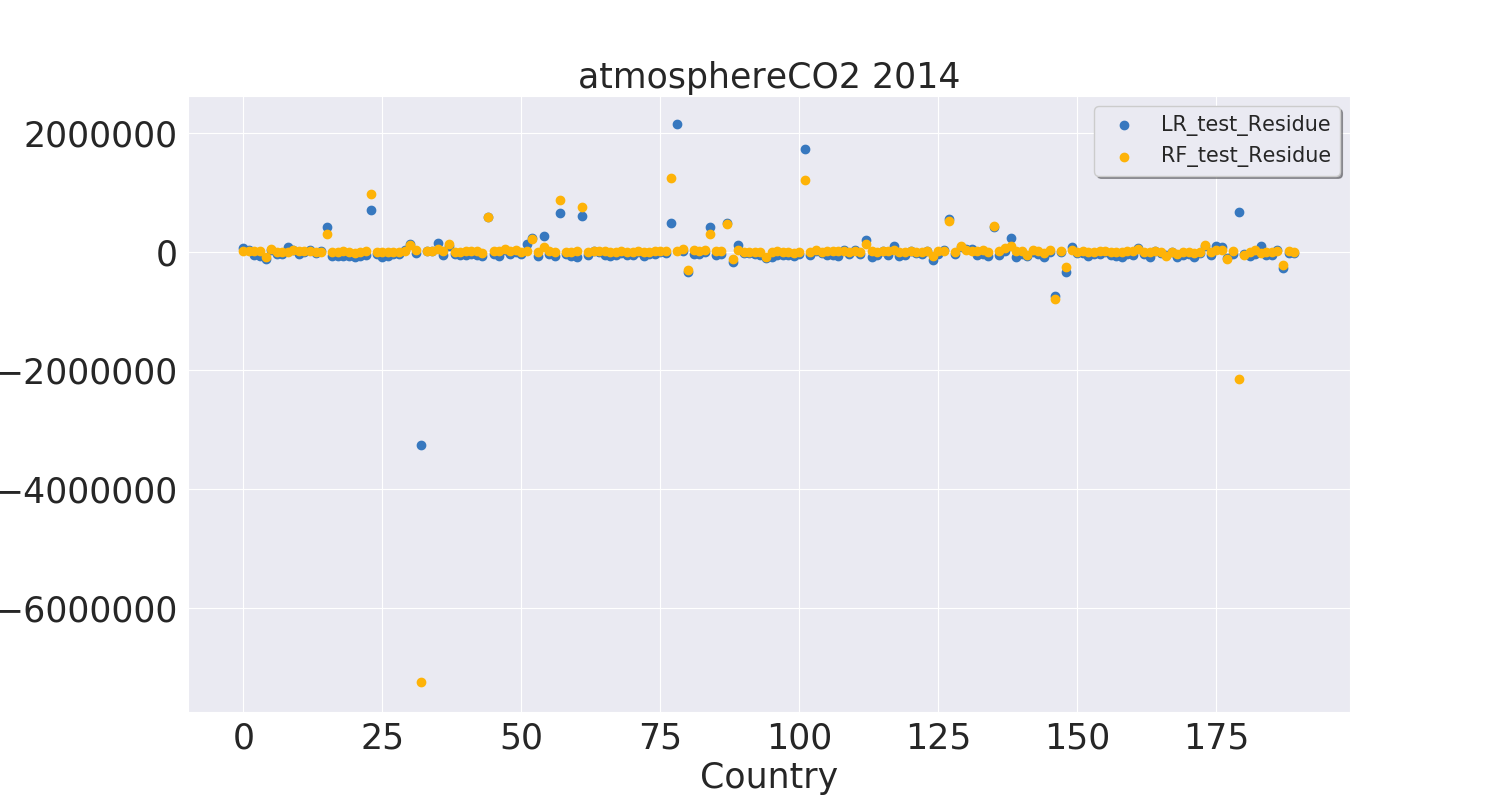
\includegraphics[width=\textwidth]{../Plots/atmosphereCO2_test_residue.png}
        \caption{Comparison between Linear Regression and Random Forest.}
        \label{fig:atmosphereCO2_test_residue}
    \end{center}
\end{figure}

A summary of performance comparison between the tested models are presented in Table \ref{PerformacneComp}.

\begin{table}[htbp!]
    \begin{center}
        \begin{tabular}{ |c|c| } 
        \hline
        Model & Root Mean Squared Error \\ 
        \hline
        Linear Regression & 326331 \\
        Decision Tree & 37946.8 \\
        Gradient Boosted Tree & 29239.1 \\
        \hline
        \end{tabular}
        \caption{Comparison of model performance using Root Mean Squared Error}
        \label{PerformanceComp}
    \end{center}
\end{table}

This comparison of performance shows the both of the machine learning methods produce predictions that are more accurate than the linear regression method by an order of magnitude, while Gradient Boosted Tree, provide the most accurate prediction out of all three. Figures \ref{fig:atmosphereCO2_test_GBT_MAPE} and \ref{fig:atmosphereCO2_test_DT_MAPE} respectively show the percentage error for Gradient Boosted Tree and Decision Tree methods, where the noticeable difference in accuracy between the two methods are displayed.

\begin{figure}[!htbp]
    \begin{center}
        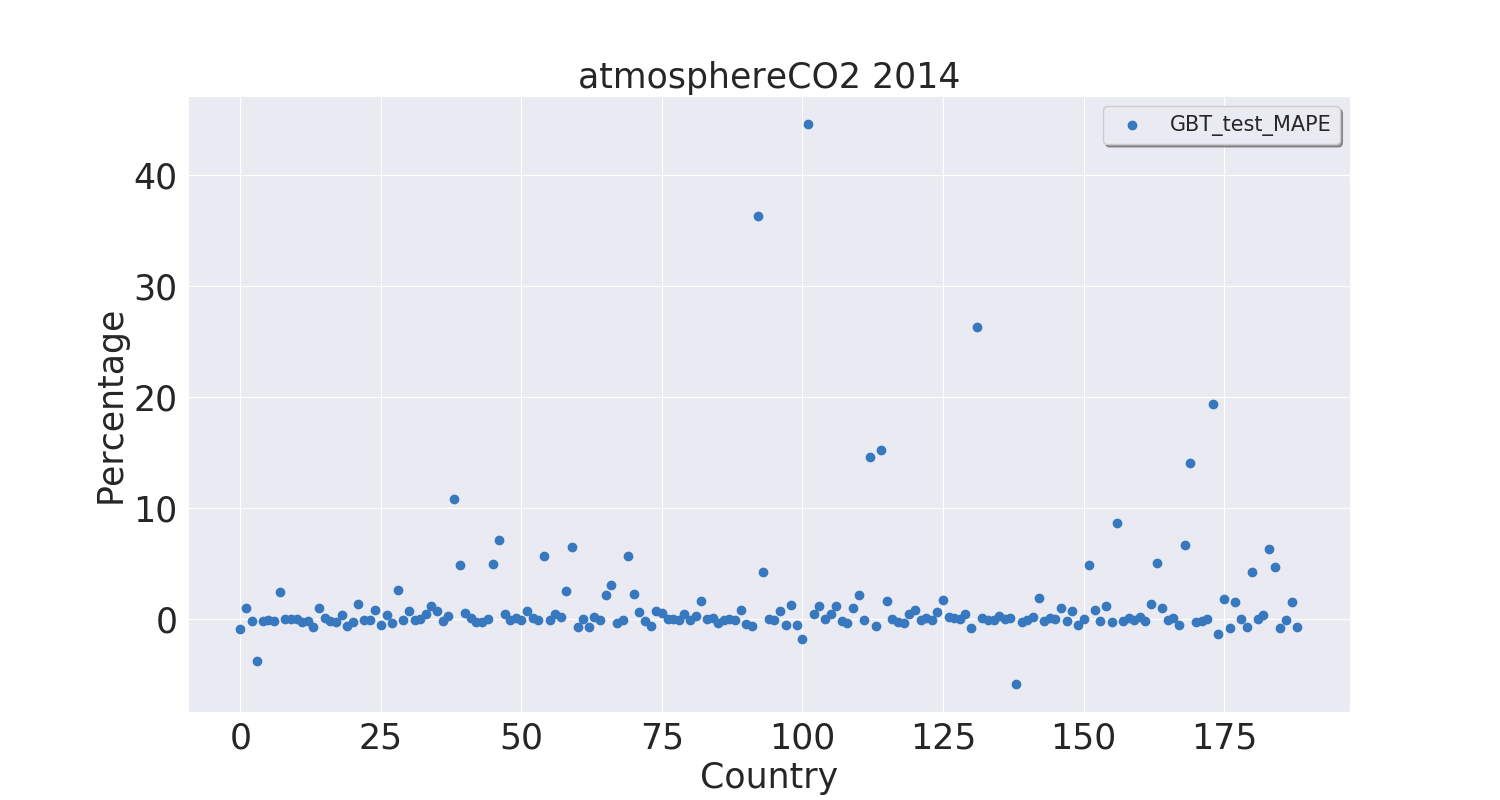
\includegraphics[width=\textwidth]{../Plots/atmosphereCO2_test_GBT_MAPE.png}
        \caption{Percentage Error from the Gradient Boosted Tree analysis.}
        \label{fig:atmosphereCO2_test_GBT_MAPE}
    \end{center}
\end{figure}

\begin{figure}[!htbp]
    \begin{center}
        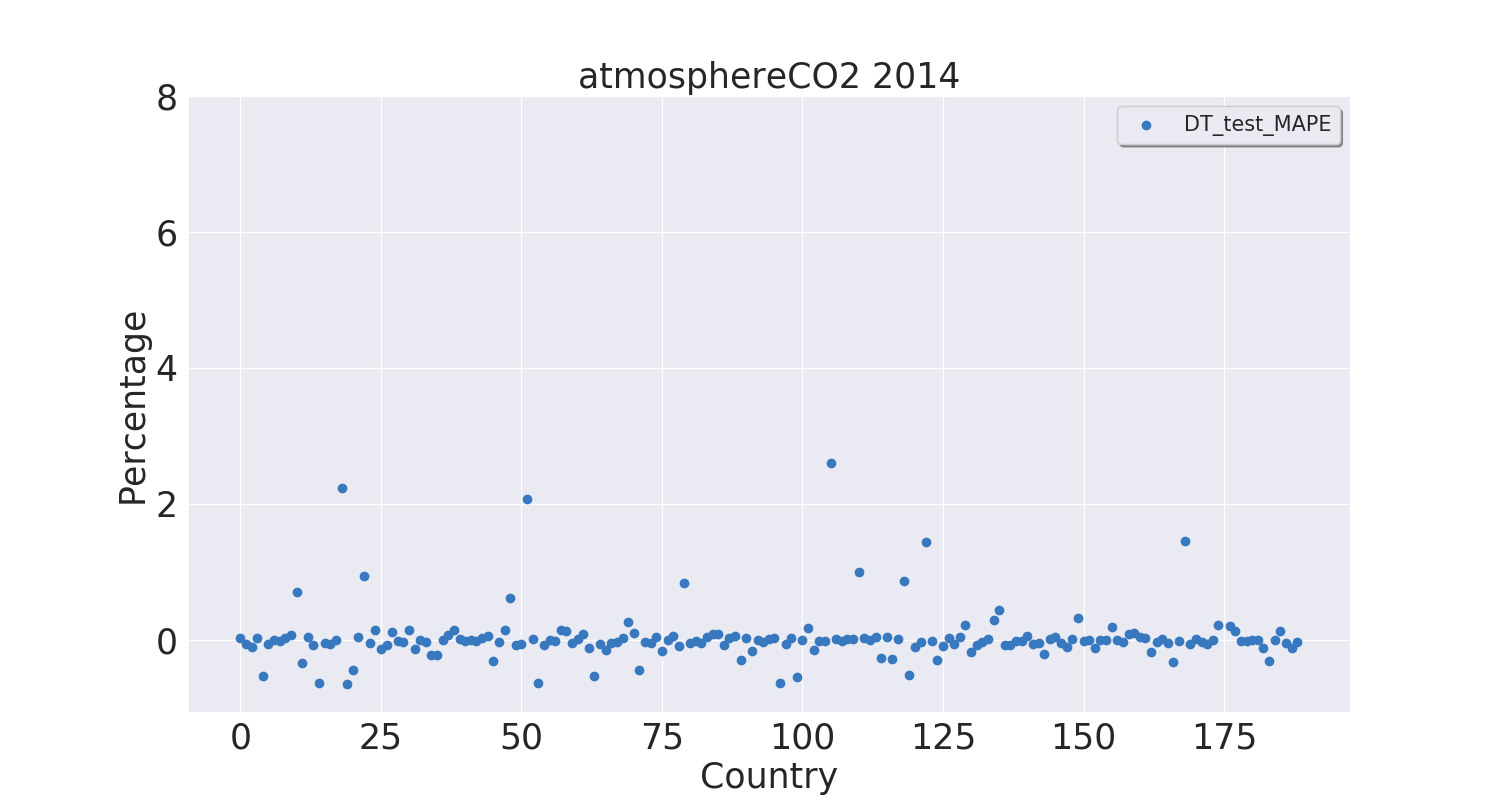
\includegraphics[width=\textwidth]{../Plots/atmosphereCO2_test_DT_MAPE.png}
        \caption{Percentage Error from the Decision Tree analysis.}
        \label{fig:atmosphereCO2_test_DT_MAPE}
    \end{center}
\end{figure}

It can be seen that most of the predictions made by the tuned Decision Tree algorithm are within one percent accurancy, with nothing surpassing four percent. Aside from achieving the best performance out of the three methods, we can also conclude that it provides quite a good level of prediction accuracy for the CO$_{2}$ emissions with the selected set of predictors. Following on from this work, more models such as Neural Networks or XGBoost can be examined to determine whether a more precise prediction can be obtained, as well as attempting to drop some predictors in the linear regression approach to see if it can perform better.

All data and source codes of this analysis can be found at \href{https://github.com/jasonyctam/WorldBankClimateChange_PySpark}{this Github repository}.

\end{document}